\documentclass[twoside]{book}

% Packages required by doxygen
\usepackage{fixltx2e}
\usepackage{calc}
\usepackage{doxygen}
\usepackage[export]{adjustbox} % also loads graphicx
\usepackage{graphicx}
\usepackage[utf8]{inputenc}
\usepackage{makeidx}
\usepackage{multicol}
\usepackage{multirow}
\PassOptionsToPackage{warn}{textcomp}
\usepackage{textcomp}
\usepackage[nointegrals]{wasysym}
\usepackage[table]{xcolor}

% Font selection
\usepackage[T1]{fontenc}
\usepackage[scaled=.90]{helvet}
\usepackage{courier}
\usepackage{amssymb}
\usepackage{sectsty}
\renewcommand{\familydefault}{\sfdefault}
\allsectionsfont{%
  \fontseries{bc}\selectfont%
  \color{darkgray}%
}
\renewcommand{\DoxyLabelFont}{%
  \fontseries{bc}\selectfont%
  \color{darkgray}%
}
\newcommand{\+}{\discretionary{\mbox{\scriptsize$\hookleftarrow$}}{}{}}

% Page & text layout
\usepackage{geometry}
\geometry{%
  a4paper,%
  top=2.5cm,%
  bottom=2.5cm,%
  left=2.5cm,%
  right=2.5cm%
}
\tolerance=750
\hfuzz=15pt
\hbadness=750
\setlength{\emergencystretch}{15pt}
\setlength{\parindent}{0cm}
\setlength{\parskip}{3ex plus 2ex minus 2ex}
\makeatletter
\renewcommand{\paragraph}{%
  \@startsection{paragraph}{4}{0ex}{-1.0ex}{1.0ex}{%
    \normalfont\normalsize\bfseries\SS@parafont%
  }%
}
\renewcommand{\subparagraph}{%
  \@startsection{subparagraph}{5}{0ex}{-1.0ex}{1.0ex}{%
    \normalfont\normalsize\bfseries\SS@subparafont%
  }%
}
\makeatother

% Headers & footers
\usepackage{fancyhdr}
\pagestyle{fancyplain}
\fancyhead[LE]{\fancyplain{}{\bfseries\thepage}}
\fancyhead[CE]{\fancyplain{}{}}
\fancyhead[RE]{\fancyplain{}{\bfseries\leftmark}}
\fancyhead[LO]{\fancyplain{}{\bfseries\rightmark}}
\fancyhead[CO]{\fancyplain{}{}}
\fancyhead[RO]{\fancyplain{}{\bfseries\thepage}}
\fancyfoot[LE]{\fancyplain{}{}}
\fancyfoot[CE]{\fancyplain{}{}}
\fancyfoot[RE]{\fancyplain{}{\bfseries\scriptsize Generated by Doxygen }}
\fancyfoot[LO]{\fancyplain{}{\bfseries\scriptsize Generated by Doxygen }}
\fancyfoot[CO]{\fancyplain{}{}}
\fancyfoot[RO]{\fancyplain{}{}}
\renewcommand{\footrulewidth}{0.4pt}
\renewcommand{\chaptermark}[1]{%
  \markboth{#1}{}%
}
\renewcommand{\sectionmark}[1]{%
  \markright{\thesection\ #1}%
}

% Indices & bibliography
\usepackage{natbib}
\usepackage[titles]{tocloft}
\setcounter{tocdepth}{3}
\setcounter{secnumdepth}{5}
\makeindex

% Hyperlinks (required, but should be loaded last)
\usepackage{ifpdf}
\ifpdf
  \usepackage[pdftex,pagebackref=true]{hyperref}
\else
  \usepackage[ps2pdf,pagebackref=true]{hyperref}
\fi
\hypersetup{%
  colorlinks=true,%
  linkcolor=blue,%
  citecolor=blue,%
  unicode%
}

% Custom commands
\newcommand{\clearemptydoublepage}{%
  \newpage{\pagestyle{empty}\cleardoublepage}%
}

\usepackage{caption}
\captionsetup{labelsep=space,justification=centering,font={bf},singlelinecheck=off,skip=4pt,position=top}

%===== C O N T E N T S =====

\begin{document}

% Titlepage & ToC
\hypersetup{pageanchor=false,
             bookmarksnumbered=true,
             pdfencoding=unicode
            }
\pagenumbering{alph}
\begin{titlepage}
\vspace*{7cm}
\begin{center}%
{\Large Figure }\\
\vspace*{1cm}
{\large Generated by Doxygen 1.8.13}\\
\end{center}
\end{titlepage}
\clearemptydoublepage
\pagenumbering{roman}
\tableofcontents
\clearemptydoublepage
\pagenumbering{arabic}
\hypersetup{pageanchor=true}

%--- Begin generated contents ---
\chapter{Hierarchical Index}
\section{Class Hierarchy}
This inheritance list is sorted roughly, but not completely, alphabetically\+:\begin{DoxyCompactList}
\item \contentsline{section}{figure}{\pageref{classfigure}}{}
\begin{DoxyCompactList}
\item \contentsline{section}{cercle}{\pageref{classcercle}}{}
\item \contentsline{section}{rectangle}{\pageref{classrectangle}}{}
\item \contentsline{section}{triangle}{\pageref{classtriangle}}{}
\end{DoxyCompactList}
\end{DoxyCompactList}

\chapter{Class Index}
\section{Class List}
Here are the classes, structs, unions and interfaces with brief descriptions\+:\begin{DoxyCompactList}
\item\contentsline{section}{\hyperlink{classcercle}{cercle} \\*La class permet d\textquotesingle{}instancier l\textquotesingle{}objet ainsi que ses méthodes }{\pageref{classcercle}}{}
\item\contentsline{section}{\hyperlink{classfigure}{figure} \\*La classe permet d\textquotesingle{}initialisé les constructeurs }{\pageref{classfigure}}{}
\item\contentsline{section}{\hyperlink{classrectangle}{rectangle} \\*La class permet d\textquotesingle{}instancier l\textquotesingle{}objet ainsi que ses méthodes }{\pageref{classrectangle}}{}
\item\contentsline{section}{\hyperlink{classtriangle}{triangle} \\*La class permet d\textquotesingle{}instancier l\textquotesingle{}objet ainsi que ses méthodes }{\pageref{classtriangle}}{}
\end{DoxyCompactList}

\chapter{File Index}
\section{File List}
Here is a list of all documented files with brief descriptions\+:\begin{DoxyCompactList}
\item\contentsline{section}{src/\hyperlink{_cercle_8h}{Cercle.\+h} \\*C\textquotesingle{}est la classe cercle }{\pageref{_cercle_8h}}{}
\item\contentsline{section}{src/\hyperlink{_figure_8h}{Figure.\+h} \\*Classe mère }{\pageref{_figure_8h}}{}
\item\contentsline{section}{src/\hyperlink{_rectangle_8h}{Rectangle.\+h} \\*C\textquotesingle{}est la classe Rectangle }{\pageref{_rectangle_8h}}{}
\item\contentsline{section}{src/\hyperlink{_triangle_8h}{Triangle.\+h} \\*C\textquotesingle{}est la classe triangle }{\pageref{_triangle_8h}}{}
\end{DoxyCompactList}

\chapter{Class Documentation}
\hypertarget{classcercle}{}\section{cercle Class Reference}
\label{classcercle}\index{cercle@{cercle}}


la class permet d\textquotesingle{}instancier l\textquotesingle{}objet ainsi que ses méthodes  




{\ttfamily \#include $<$Cercle.\+h$>$}



Inheritance diagram for cercle\+:
\nopagebreak
\begin{figure}[H]
\begin{center}
\leavevmode
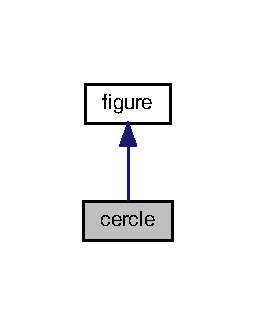
\includegraphics[width=123pt]{classcercle__inherit__graph}
\end{center}
\end{figure}


Collaboration diagram for cercle\+:
\nopagebreak
\begin{figure}[H]
\begin{center}
\leavevmode
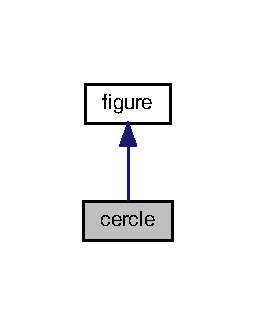
\includegraphics[width=123pt]{classcercle__coll__graph}
\end{center}
\end{figure}
\subsection*{Public Member Functions}
\begin{DoxyCompactItemize}
\item 
float \hyperlink{classcercle_a6d52510464c33891cac6bf7580d559da}{calc\+Surface} (float \+\_\+rayon)
\begin{DoxyCompactList}\small\item\em calc\+Surface \end{DoxyCompactList}\item 
float \hyperlink{classcercle_a5f309ec11993e49a8f9009ddb797dcd0}{calc\+Perim} (float \+\_\+rayon)
\begin{DoxyCompactList}\small\item\em calc\+Perim \end{DoxyCompactList}\end{DoxyCompactItemize}
\subsection*{Public Attributes}
\begin{DoxyCompactItemize}
\item 
\mbox{\Hypertarget{classcercle_aed10f4294672b96cd33ae2826a316273}\label{classcercle_aed10f4294672b96cd33ae2826a316273}} 
float {\bfseries Rayon}
\end{DoxyCompactItemize}


\subsection{Detailed Description}
la class permet d\textquotesingle{}instancier l\textquotesingle{}objet ainsi que ses méthodes 

\subsection{Member Function Documentation}
\mbox{\Hypertarget{classcercle_a5f309ec11993e49a8f9009ddb797dcd0}\label{classcercle_a5f309ec11993e49a8f9009ddb797dcd0}} 
\index{cercle@{cercle}!calc\+Perim@{calc\+Perim}}
\index{calc\+Perim@{calc\+Perim}!cercle@{cercle}}
\subsubsection{\texorpdfstring{calc\+Perim()}{calcPerim()}}
{\footnotesize\ttfamily float cercle\+::calc\+Perim (\begin{DoxyParamCaption}\item[{float}]{\+\_\+rayon }\end{DoxyParamCaption})}



calc\+Perim 


\begin{DoxyParams}{Parameters}
{\em \+\_\+rayon} & -\/$>$ ce qu\textquotesingle{}on donne en param pour les calculs(le rayon du cercle) \\
\hline
\end{DoxyParams}
\begin{DoxyReturn}{Returns}
ça retourne le perimetre du cercle 
\end{DoxyReturn}
\mbox{\Hypertarget{classcercle_a6d52510464c33891cac6bf7580d559da}\label{classcercle_a6d52510464c33891cac6bf7580d559da}} 
\index{cercle@{cercle}!calc\+Surface@{calc\+Surface}}
\index{calc\+Surface@{calc\+Surface}!cercle@{cercle}}
\subsubsection{\texorpdfstring{calc\+Surface()}{calcSurface()}}
{\footnotesize\ttfamily float cercle\+::calc\+Surface (\begin{DoxyParamCaption}\item[{float}]{\+\_\+rayon }\end{DoxyParamCaption})}



calc\+Surface 


\begin{DoxyParams}{Parameters}
{\em \+\_\+rayon} & -\/$>$ ce qu\textquotesingle{}on donne en param pour les calculs(le rayon du cercle) \\
\hline
\end{DoxyParams}
\begin{DoxyReturn}{Returns}
ça retourne la Surface du cercle 
\end{DoxyReturn}


The documentation for this class was generated from the following files\+:\begin{DoxyCompactItemize}
\item 
src/\hyperlink{_cercle_8h}{Cercle.\+h}\item 
src/Cercle.\+cpp\end{DoxyCompactItemize}

\hypertarget{classfigure}{}\section{figure Class Reference}
\label{classfigure}\index{figure@{figure}}


la classe permet d\textquotesingle{}initialisé les constructeurs  




{\ttfamily \#include $<$Figure.\+h$>$}



Inheritance diagram for figure\+:
\nopagebreak
\begin{figure}[H]
\begin{center}
\leavevmode
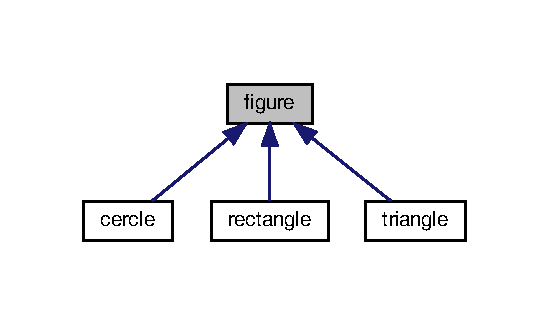
\includegraphics[width=264pt]{classfigure__inherit__graph}
\end{center}
\end{figure}
\subsection*{Public Member Functions}
\begin{DoxyCompactItemize}
\item 
virtual int \hyperlink{classfigure_a168accd9182dbbef2a580c5e1c34d12e}{calc\+Surface} ()
\begin{DoxyCompactList}\small\item\em calcul de la surface \end{DoxyCompactList}\item 
virtual int \hyperlink{classfigure_afc1d57fa737d39192a0c00125c4cda19}{calc\+Perim} ()
\begin{DoxyCompactList}\small\item\em calcul du perimetre \end{DoxyCompactList}\end{DoxyCompactItemize}


\subsection{Detailed Description}
la classe permet d\textquotesingle{}initialisé les constructeurs 

\subsection{Member Function Documentation}
\mbox{\Hypertarget{classfigure_afc1d57fa737d39192a0c00125c4cda19}\label{classfigure_afc1d57fa737d39192a0c00125c4cda19}} 
\index{figure@{figure}!calc\+Perim@{calc\+Perim}}
\index{calc\+Perim@{calc\+Perim}!figure@{figure}}
\subsubsection{\texorpdfstring{calc\+Perim()}{calcPerim()}}
{\footnotesize\ttfamily int figure\+::calc\+Perim (\begin{DoxyParamCaption}{ }\end{DoxyParamCaption})\hspace{0.3cm}{\ttfamily [virtual]}}



calcul du perimetre 


\begin{DoxyParams}{Parameters}
{\em aucun} & paramètres car c\textquotesingle{}est la classe parent que l\textquotesingle{}on instancie jamais \\
\hline
\end{DoxyParams}
\begin{DoxyReturn}{Returns}
ça ne retourne rien 
\end{DoxyReturn}
\mbox{\Hypertarget{classfigure_a168accd9182dbbef2a580c5e1c34d12e}\label{classfigure_a168accd9182dbbef2a580c5e1c34d12e}} 
\index{figure@{figure}!calc\+Surface@{calc\+Surface}}
\index{calc\+Surface@{calc\+Surface}!figure@{figure}}
\subsubsection{\texorpdfstring{calc\+Surface()}{calcSurface()}}
{\footnotesize\ttfamily int figure\+::calc\+Surface (\begin{DoxyParamCaption}{ }\end{DoxyParamCaption})\hspace{0.3cm}{\ttfamily [virtual]}}



calcul de la surface 


\begin{DoxyParams}{Parameters}
{\em aucun} & paramètres car c\textquotesingle{}est la classe parent que l\textquotesingle{}on instancie jamais \\
\hline
\end{DoxyParams}
\begin{DoxyReturn}{Returns}
ça ne retourne rien 
\end{DoxyReturn}


The documentation for this class was generated from the following files\+:\begin{DoxyCompactItemize}
\item 
src/\hyperlink{_figure_8h}{Figure.\+h}\item 
src/Figure.\+cpp\end{DoxyCompactItemize}

\hypertarget{classrectangle}{}\section{rectangle Class Reference}
\label{classrectangle}\index{rectangle@{rectangle}}


la class permet d\textquotesingle{}instancier l\textquotesingle{}objet ainsi que ses méthodes  




{\ttfamily \#include $<$Rectangle.\+h$>$}



Inheritance diagram for rectangle\+:
\nopagebreak
\begin{figure}[H]
\begin{center}
\leavevmode
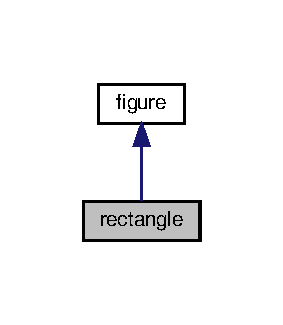
\includegraphics[width=136pt]{classrectangle__inherit__graph}
\end{center}
\end{figure}


Collaboration diagram for rectangle\+:
\nopagebreak
\begin{figure}[H]
\begin{center}
\leavevmode
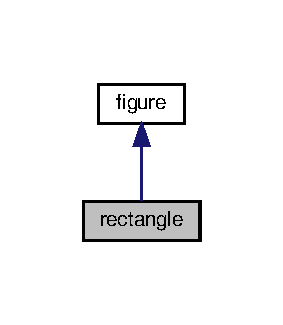
\includegraphics[width=136pt]{classrectangle__coll__graph}
\end{center}
\end{figure}
\subsection*{Public Member Functions}
\begin{DoxyCompactItemize}
\item 
int \hyperlink{classrectangle_a26f1b435a0ef3f92dbad8c24a7d83d77}{calc\+Surface} (int \+\_\+\+Longeur, int \+\_\+\+Largeur)
\begin{DoxyCompactList}\small\item\em calc\+Surface \end{DoxyCompactList}\item 
int \hyperlink{classrectangle_adb98c249f2c6a0910013869c9b698b1a}{calc\+Perim} (int \+\_\+\+Longeur, int \+\_\+\+Largeur)
\begin{DoxyCompactList}\small\item\em calc\+Perim \end{DoxyCompactList}\end{DoxyCompactItemize}
\subsection*{Public Attributes}
\begin{DoxyCompactItemize}
\item 
\mbox{\Hypertarget{classrectangle_aa08d37496ef07314559fb6b8e172a9c0}\label{classrectangle_aa08d37496ef07314559fb6b8e172a9c0}} 
int {\bfseries Longeur}
\item 
\mbox{\Hypertarget{classrectangle_a207facc5dabb41085bfb74b73a12526d}\label{classrectangle_a207facc5dabb41085bfb74b73a12526d}} 
int {\bfseries Largeur}
\end{DoxyCompactItemize}


\subsection{Detailed Description}
la class permet d\textquotesingle{}instancier l\textquotesingle{}objet ainsi que ses méthodes 

\subsection{Member Function Documentation}
\mbox{\Hypertarget{classrectangle_adb98c249f2c6a0910013869c9b698b1a}\label{classrectangle_adb98c249f2c6a0910013869c9b698b1a}} 
\index{rectangle@{rectangle}!calc\+Perim@{calc\+Perim}}
\index{calc\+Perim@{calc\+Perim}!rectangle@{rectangle}}
\subsubsection{\texorpdfstring{calc\+Perim()}{calcPerim()}}
{\footnotesize\ttfamily int rectangle\+::calc\+Perim (\begin{DoxyParamCaption}\item[{int}]{\+\_\+\+Longeur,  }\item[{int}]{\+\_\+\+Largeur }\end{DoxyParamCaption})}



calc\+Perim 


\begin{DoxyParams}{Parameters}
{\em \+\_\+\+Longeur} & -\/$>$ ce qu\textquotesingle{}on donne en param pour les calculs \\
\hline
{\em \+\_\+\+Largeur} & -\/$>$ ce qu\textquotesingle{}on donne en param pour les calculs \\
\hline
\end{DoxyParams}
\begin{DoxyReturn}{Returns}
ça retourne le calcul du perimetre des deux int 
\end{DoxyReturn}
\mbox{\Hypertarget{classrectangle_a26f1b435a0ef3f92dbad8c24a7d83d77}\label{classrectangle_a26f1b435a0ef3f92dbad8c24a7d83d77}} 
\index{rectangle@{rectangle}!calc\+Surface@{calc\+Surface}}
\index{calc\+Surface@{calc\+Surface}!rectangle@{rectangle}}
\subsubsection{\texorpdfstring{calc\+Surface()}{calcSurface()}}
{\footnotesize\ttfamily int rectangle\+::calc\+Surface (\begin{DoxyParamCaption}\item[{int}]{\+\_\+\+Longeur,  }\item[{int}]{\+\_\+\+Largeur }\end{DoxyParamCaption})}



calc\+Surface 


\begin{DoxyParams}{Parameters}
{\em \+\_\+\+Longeur} & -\/$>$ ce qu\textquotesingle{}on donne en param pour les calculs \\
\hline
{\em \+\_\+\+Largeur} & -\/$>$ ce qu\textquotesingle{}on donne en param pour les calculs \\
\hline
\end{DoxyParams}
\begin{DoxyReturn}{Returns}
ça retourne la Surface de deux int 
\end{DoxyReturn}


The documentation for this class was generated from the following files\+:\begin{DoxyCompactItemize}
\item 
src/\hyperlink{_rectangle_8h}{Rectangle.\+h}\item 
src/Rectangle.\+cpp\end{DoxyCompactItemize}

\hypertarget{classtriangle}{}\section{triangle Class Reference}
\label{classtriangle}\index{triangle@{triangle}}


la class permet d\textquotesingle{}instancier l\textquotesingle{}objet ainsi que ses méthodes  




{\ttfamily \#include $<$Triangle.\+h$>$}



Inheritance diagram for triangle\+:
\nopagebreak
\begin{figure}[H]
\begin{center}
\leavevmode
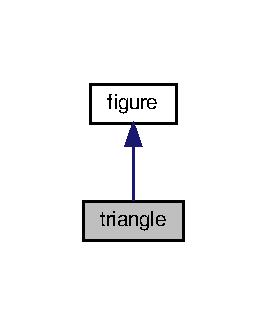
\includegraphics[width=128pt]{classtriangle__inherit__graph}
\end{center}
\end{figure}


Collaboration diagram for triangle\+:
\nopagebreak
\begin{figure}[H]
\begin{center}
\leavevmode
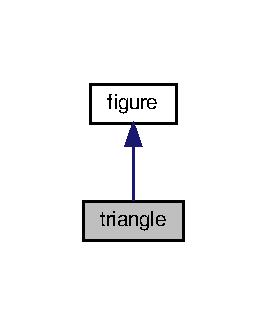
\includegraphics[width=128pt]{classtriangle__coll__graph}
\end{center}
\end{figure}
\subsection*{Public Member Functions}
\begin{DoxyCompactItemize}
\item 
int \hyperlink{classtriangle_ac5fc18c9689b3cf055b431cfd189fe3b}{calc\+Surface} (int \+\_\+cote1, int \+\_\+cote2, int \+\_\+cote3)
\begin{DoxyCompactList}\small\item\em calc\+Surface \end{DoxyCompactList}\item 
int \hyperlink{classtriangle_add93fe57e11592724508a1236b1178bf}{calc\+Perim} (int \+\_\+hauteur, int \+\_\+base)
\begin{DoxyCompactList}\small\item\em calc\+Surface \end{DoxyCompactList}\end{DoxyCompactItemize}
\subsection*{Public Attributes}
\begin{DoxyCompactItemize}
\item 
\mbox{\Hypertarget{classtriangle_aa241ebfeffaa2380d7be72c0d11de72d}\label{classtriangle_aa241ebfeffaa2380d7be72c0d11de72d}} 
int {\bfseries cote1}
\item 
\mbox{\Hypertarget{classtriangle_a323803e1c48fb9dace4f57d77072902e}\label{classtriangle_a323803e1c48fb9dace4f57d77072902e}} 
int {\bfseries cote2}
\item 
\mbox{\Hypertarget{classtriangle_ad72ee9ea67e6042ad0a87b9ba791a9d6}\label{classtriangle_ad72ee9ea67e6042ad0a87b9ba791a9d6}} 
int {\bfseries cote3}
\item 
\mbox{\Hypertarget{classtriangle_a537cf5aab61c3e499414a8e8b32aee0d}\label{classtriangle_a537cf5aab61c3e499414a8e8b32aee0d}} 
int {\bfseries hauteur}
\item 
\mbox{\Hypertarget{classtriangle_a2b3dabbc0590c1b43f52642094ac253c}\label{classtriangle_a2b3dabbc0590c1b43f52642094ac253c}} 
int {\bfseries base}
\end{DoxyCompactItemize}


\subsection{Detailed Description}
la class permet d\textquotesingle{}instancier l\textquotesingle{}objet ainsi que ses méthodes 

\subsection{Member Function Documentation}
\mbox{\Hypertarget{classtriangle_add93fe57e11592724508a1236b1178bf}\label{classtriangle_add93fe57e11592724508a1236b1178bf}} 
\index{triangle@{triangle}!calc\+Perim@{calc\+Perim}}
\index{calc\+Perim@{calc\+Perim}!triangle@{triangle}}
\subsubsection{\texorpdfstring{calc\+Perim()}{calcPerim()}}
{\footnotesize\ttfamily int triangle\+::calc\+Perim (\begin{DoxyParamCaption}\item[{int}]{\+\_\+hauteur,  }\item[{int}]{\+\_\+base }\end{DoxyParamCaption})}



calc\+Surface 


\begin{DoxyParams}{Parameters}
{\em \+\_\+hauteur} & -\/$>$ ce qu\textquotesingle{}on donne en param pour les calculs \\
\hline
{\em \+\_\+base} & -\/$>$ ce qu\textquotesingle{}on donne en param pour les calculs \\
\hline
\end{DoxyParams}
\begin{DoxyReturn}{Returns}
ça retourne le calcul du perimètre 
\end{DoxyReturn}
\mbox{\Hypertarget{classtriangle_ac5fc18c9689b3cf055b431cfd189fe3b}\label{classtriangle_ac5fc18c9689b3cf055b431cfd189fe3b}} 
\index{triangle@{triangle}!calc\+Surface@{calc\+Surface}}
\index{calc\+Surface@{calc\+Surface}!triangle@{triangle}}
\subsubsection{\texorpdfstring{calc\+Surface()}{calcSurface()}}
{\footnotesize\ttfamily int triangle\+::calc\+Surface (\begin{DoxyParamCaption}\item[{int}]{\+\_\+cote1,  }\item[{int}]{\+\_\+cote2,  }\item[{int}]{\+\_\+cote3 }\end{DoxyParamCaption})}



calc\+Surface 


\begin{DoxyParams}{Parameters}
{\em \+\_\+cote1} & -\/$>$ ce qu\textquotesingle{}on donne en param pour les calculs \\
\hline
{\em \+\_\+cote2} & -\/$>$ ce qu\textquotesingle{}on donne en param pour les calculs \\
\hline
{\em \+\_\+cote3} & -\/$>$ ce qu\textquotesingle{}on donne en param pour les calculs \\
\hline
\end{DoxyParams}
\begin{DoxyReturn}{Returns}
ça retourne la Surface 
\end{DoxyReturn}


The documentation for this class was generated from the following files\+:\begin{DoxyCompactItemize}
\item 
src/\hyperlink{_triangle_8h}{Triangle.\+h}\item 
src/Triangle.\+cpp\end{DoxyCompactItemize}

\chapter{File Documentation}
\hypertarget{_cercle_8h}{}\section{src/\+Cercle.h File Reference}
\label{_cercle_8h}\index{src/\+Cercle.\+h@{src/\+Cercle.\+h}}


C\textquotesingle{}est la classe cercle.  


{\ttfamily \#include $<$iostream$>$}\newline
{\ttfamily \#include \char`\"{}Figure.\+h\char`\"{}}\newline
Include dependency graph for Cercle.\+h\+:
\nopagebreak
\begin{figure}[H]
\begin{center}
\leavevmode
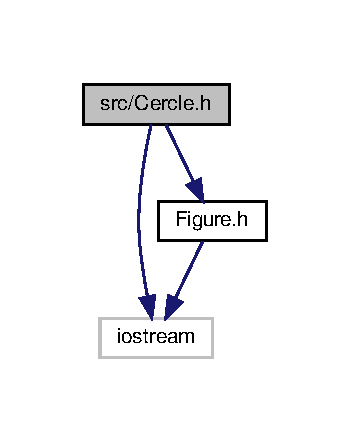
\includegraphics[width=168pt]{_cercle_8h__incl}
\end{center}
\end{figure}
\subsection*{Classes}
\begin{DoxyCompactItemize}
\item 
class \hyperlink{classcercle}{cercle}
\begin{DoxyCompactList}\small\item\em la class permet d\textquotesingle{}instancier l\textquotesingle{}objet ainsi que ses méthodes \end{DoxyCompactList}\end{DoxyCompactItemize}


\subsection{Detailed Description}
C\textquotesingle{}est la classe cercle. 

\begin{DoxyAuthor}{Author}
Maxence 
\end{DoxyAuthor}
\begin{DoxyVersion}{Version}
1.\+0 
\end{DoxyVersion}

\hypertarget{_figure_8h}{}\section{src/\+Figure.h File Reference}
\label{_figure_8h}\index{src/\+Figure.\+h@{src/\+Figure.\+h}}


classe mère  


{\ttfamily \#include $<$iostream$>$}\newline
Include dependency graph for Figure.\+h\+:
\nopagebreak
\begin{figure}[H]
\begin{center}
\leavevmode
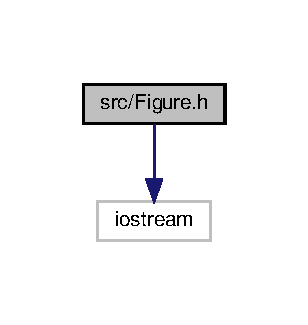
\includegraphics[width=148pt]{_figure_8h__incl}
\end{center}
\end{figure}
This graph shows which files directly or indirectly include this file\+:
\nopagebreak
\begin{figure}[H]
\begin{center}
\leavevmode
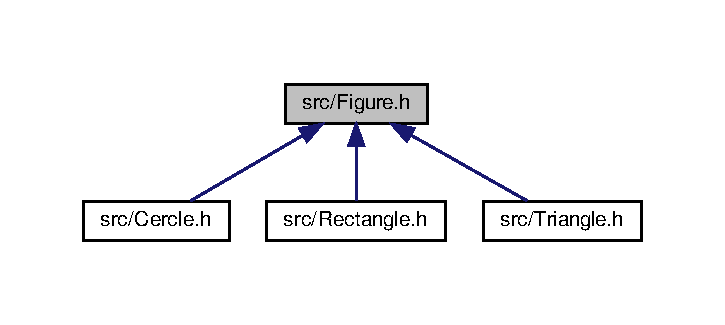
\includegraphics[width=348pt]{_figure_8h__dep__incl}
\end{center}
\end{figure}
\subsection*{Classes}
\begin{DoxyCompactItemize}
\item 
class \hyperlink{classfigure}{figure}
\begin{DoxyCompactList}\small\item\em la classe permet d\textquotesingle{}initialisé les constructeurs \end{DoxyCompactList}\end{DoxyCompactItemize}


\subsection{Detailed Description}
classe mère 

\begin{DoxyAuthor}{Author}
Maxence 
\end{DoxyAuthor}
\begin{DoxyVersion}{Version}
1.\+0 
\end{DoxyVersion}

\hypertarget{_rectangle_8h}{}\section{src/\+Rectangle.h File Reference}
\label{_rectangle_8h}\index{src/\+Rectangle.\+h@{src/\+Rectangle.\+h}}


C\textquotesingle{}est la classe Rectangle.  


{\ttfamily \#include $<$iostream$>$}\newline
{\ttfamily \#include \char`\"{}Figure.\+h\char`\"{}}\newline
Include dependency graph for Rectangle.\+h\+:
\nopagebreak
\begin{figure}[H]
\begin{center}
\leavevmode
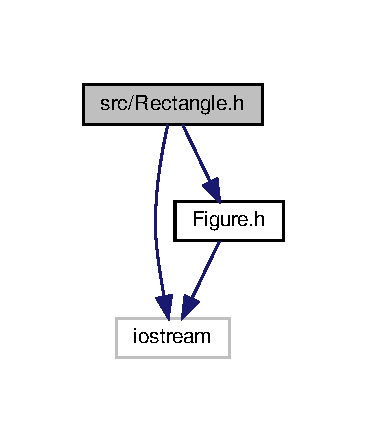
\includegraphics[width=176pt]{_rectangle_8h__incl}
\end{center}
\end{figure}
\subsection*{Classes}
\begin{DoxyCompactItemize}
\item 
class \hyperlink{classrectangle}{rectangle}
\begin{DoxyCompactList}\small\item\em la class permet d\textquotesingle{}instancier l\textquotesingle{}objet ainsi que ses méthodes \end{DoxyCompactList}\end{DoxyCompactItemize}


\subsection{Detailed Description}
C\textquotesingle{}est la classe Rectangle. 

\begin{DoxyAuthor}{Author}
Maxence 
\end{DoxyAuthor}
\begin{DoxyVersion}{Version}
1.\+0 
\end{DoxyVersion}

\hypertarget{_triangle_8h}{}\section{src/\+Triangle.h File Reference}
\label{_triangle_8h}\index{src/\+Triangle.\+h@{src/\+Triangle.\+h}}


C\textquotesingle{}est la classe triangle.  


{\ttfamily \#include $<$iostream$>$}\newline
{\ttfamily \#include \char`\"{}Figure.\+h\char`\"{}}\newline
Include dependency graph for Triangle.\+h\+:
\nopagebreak
\begin{figure}[H]
\begin{center}
\leavevmode
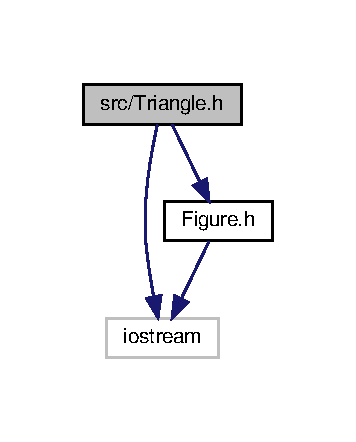
\includegraphics[width=171pt]{_triangle_8h__incl}
\end{center}
\end{figure}
\subsection*{Classes}
\begin{DoxyCompactItemize}
\item 
class \hyperlink{classtriangle}{triangle}
\begin{DoxyCompactList}\small\item\em la class permet d\textquotesingle{}instancier l\textquotesingle{}objet ainsi que ses méthodes \end{DoxyCompactList}\end{DoxyCompactItemize}


\subsection{Detailed Description}
C\textquotesingle{}est la classe triangle. 

\begin{DoxyAuthor}{Author}
Maxence 
\end{DoxyAuthor}
\begin{DoxyVersion}{Version}
1.\+0 
\end{DoxyVersion}

%--- End generated contents ---

% Index
\backmatter
\newpage
\phantomsection
\clearemptydoublepage
\addcontentsline{toc}{chapter}{Index}
\printindex

\end{document}
